\documentclass[12pt]{article}
\usepackage{graphicx}
\usepackage{amsmath}
\usepackage{mathtools}
\usepackage{gensymb}
\usepackage{amssymb}
\usepackage{tikz}
\usetikzlibrary{arrows,shapes,automata,petri,positioning,calc}
\usepackage{hyperref}
\usepackage{tikz}
\usetikzlibrary{matrix,calc}
\usepackage[margin=0.5in]{geometry}

\providecommand{\norm}[1]{\left\lVert#1\right\rVert}
\newcommand{\myvec}[1]{\ensuremath{\begin{pmatrix}#1\end{pmatrix}}}
\let\vec\mathbf
%\providecommand $${\norm}[1]{\left\lVert#1\right\rVert}$$
\providecommand{\abs}[1]{\left\vert#1\right\vert}
\let\vec\mathbf

\newcommand{\mydet}[1]{\ensuremath{\begin{vmatrix}#1\end{vmatrix}}}
\providecommand{\brak}[1]{\ensuremath{\left(#1\right)}}
\providecommand{\lbrak}[1]{\ensuremath{\left(#1\right.}}
\providecommand{\rbrak}[1]{\ensuremath{\left.#1\right)}}
\providecommand{\sbrak}[1]{\ensuremath{{}\left[#1\right]}}

\providecommand{\brak}[1]{\ensuremath{\left(#1\right)}}
\providecommand{\norm}[1]{\left\lVert#1\right\rVert}
\newcommand{\solution}{\noindent \textbf{Solution: }}

\let\vec\mathbf
\def\inputGnumericTable{}
\usepackage{color}                                            %%
    \usepackage{array}                                            %%
    \usepackage{longtable}                                        %%
    \usepackage{calc}                                             %%
    \usepackage{multirow}                                         %%
    \usepackage{hhline}                                           %%
    \usepackage{ifthen}
\usepackage{array}
\usepackage{amsmath}   % for having text in math mode
\usepackage{listings}
\lstset{
language=tex,
frame=single, 
breaklines=true
}
\newenvironment{Figure}
  {\par\medskip\noindent\minipage{\linewidth}}
  {\endminipage\par\medskip}
\begin{document}
\begin{center}
\textbf\large{CLASS-9\\CHAPTER-10 \\ CIRCLES}

\end{center}
\section*{Excercise 10.6}

Q1. Prove that the line of centres of two intersecting circles subtends equal angles at the two points of intersection.
\section*{\large Solution}:
\begin{figure}[h!]
\centering
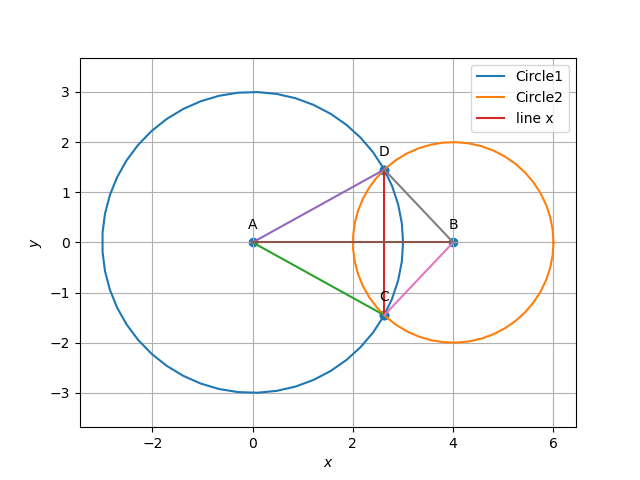
\includegraphics[width=\columnwidth]{figs/circle3.png}
\caption{}
\label{fig:Fig1}
\end{figure}


\section*{\large Construction}:

\begin{table}[h!]
	\small
	\centering
	%\subimport{../tables/}{table1.tex}
     %%%%%%%%%%%%%%%%%%%%%%%%%%%%%%%%%%%%%%%%%%%%%%%%%%%%%%%%%%%%%%%%%%%%%%
%%                                                                  %%
%%  This is the header of a LaTeX2e file exported from Gnumeric.    %%
%%                                                                  %%
%%  This file can be compiled as it stands or included in another   %%
%%  LaTeX document. The table is based on the longtable package so  %%
%%  the longtable options (headers, footers...) can be set in the   %%
%%  preamble section below (see PRAMBLE).                           %%
%%                                                                  %%
%%  To include the file in another, the following two lines must be %%
%%  in the including file:                                          %%
%%        \def\inputGnumericTable{}                                 %%
%%  at the beginning of the file and:                               %%
%%        \input{name-of-this-file.tex}                             %%
%%  where the table is to be placed. Note also that the including   %%
%%  file must use the following packages for the table to be        %%
%%  rendered correctly:                                             %%
%%    \usepackage[latin1]{inputenc}                                 %%
%%    \usepackage{color}                                            %%
%%    \usepackage{array}                                            %%
%%    \usepackage{longtable}                                        %%
%%    \usepackage{calc}                                             %%
%%    \usepackage{multirow}                                         %%
%%    \usepackage{hhline}                                           %%
%%    \usepackage{ifthen}                                           %%
%%  optionally (for landscape tables embedded in another document): %%
%%    \usepackage{lscape}                                           %%
%%                                                                  %%
%%%%%%%%%%%%%%%%%%%%%%%%%%%%%%%%%%%%%%%%%%%%%%%%%%%%%%%%%%%%%%%%%%%%%



%%  This section checks if we are begin input into another file or  %%
%%  the file will be compiled alone. First use a macro taken from   %%
%%  the TeXbook ex 7.7 (suggestion of Han-Wen Nienhuys).            %%
\def\ifundefined#1{\expandafter\ifx\csname#1\endcsname\relax}


%%  Check for the \def token for inputed files. If it is not        %%
%%  defined, the file will be processed as a standalone and the     %%
%%  preamble will be used.                                          %%
\ifundefined{inputGnumericTable}

%%  We must be able to close or not the document at the end.        %%
	\def\gnumericTableEnd{\end{document}}


%%%%%%%%%%%%%%%%%%%%%%%%%%%%%%%%%%%%%%%%%%%%%%%%%%%%%%%%%%%%%%%%%%%%%%
%%                                                                  %%
%%  This is the PREAMBLE. Change these values to get the right      %%
%%  paper size and other niceties.                                  %%
%%                                                                  %%
%%%%%%%%%%%%%%%%%%%%%%%%%%%%%%%%%%%%%%%%%%%%%%%%%%%%%%%%%%%%%%%%%%%%%%

	\documentclass[12pt%
			  %,landscape%
                    ]{report}
       \usepackage[latin1]{inputenc}
       \usepackage{fullpage}
       \usepackage{color}
       \usepackage{array}
       \usepackage{longtable}
       \usepackage{calc}
       \usepackage{multirow}
       \usepackage{hhline}
       \usepackage{ifthen}
       \usepackage{gensymb}
       \usepackage{graphicx}
\usepackage{amsmath}
\usepackage{mathtools}
\newcommand{\mydet}[1]{\ensuremath{\begin{vmatrix}#1\end{vmatrix}}}
\providecommand{\brak}[1]{\ensuremath{\left(#1\right)}}
\providecommand{\norm}[1]{\left\lVert#1\right\rVert}
\newcommand{\solution}{\noindent \textbf{Solution: }}
\newcommand{\myvec}[1]{\ensuremath{\begin{pmatrix}#1\end{pmatrix}}}
\let\vec\mathbf
	\begin{document}


%%  End of the preamble for the standalone. The next section is for %%
%%  documents which are included into other LaTeX2e files.          %%
\else

%%  We are not a stand alone document. For a regular able, we will %%
%%  have no preamble and only define the closing to mean nothing.   %%
    \def\gnumericTableEnd{}

%%  If we want landscape mode in an embedded document, comment out  %%
%%  the line above and uncomment the two below. The table will      %%
%%  begin on a new page and run in landscape mode.                  %%
%       \def\gnumericTableEnd{\end{landscape}}
%       \begin{landscape}


%%  End of the else clause for this file being \input.              %%
\fi

%%%%%%%%%%%%%%%%%%%%%%%%%%%%%%%%%%%%%%%%%%%%%%%%%%%%%%%%%%%%%%%%%%%%%%
%%                                                                  %%
%%  The rest is the gnumeric table, except for the closing          %%
%%  statement. Changes below will alter the table's appearance.     %%
%%                                                                  %%
%%%%%%%%%%%%%%%%%%%%%%%%%%%%%%%%%%%%%%%%%%%%%%%%%%%%%%%%%%%%%%%%%%%%%%
\providecommand{\gnumericmathit}[1]{#1} 
%%  Uncomment the next line if you would like your numbers to be in %%
%%  italics if they are italizised in the gnumeric table.           %%
%\renewcommand{\gnumericmathit}[1]{\mathit{#1}}
\providecommand{\gnumericPB}[1]%
{\let\gnumericTemp=\\#1\let\\=\gnumericTemp\hspace{0pt}}
 \ifundefined{gnumericTableWidthDefined}
        \newlength{\gnumericTableWidth}
        \newlength{\gnumericTableWidthComplete}
        \newlength{\gnumericMultiRowLength}
        \global\def\gnumericTableWidthDefined{}
 \fi
%% The following setting protects this code from babel shorthands.  %%
 \ifthenelse{\isundefined{\languageshorthands}}{}{\languageshorthands{english}}
%%  The default table format retains the relative column widths of  %%
%%  gnumeric. They can easily be changed to c, r or l. In that case %%
%%  you may want to comment out the next line and uncomment the one %%
%%  thereafter                                                      %%
\providecommand\gnumbox{\makebox[0pt]}
%%\providecommand\gnumbox[1][]{\makebox}

%% to adjust positions in multirow situations                       %%
\setlength{\bigstrutjot}{\jot}
\setlength{\extrarowheight}{\doublerulesep}

%%  The \setlongtables command keeps column widths the same across  %%
%%  pages. Simply comment out next line for varying column widths.  %%
\setlongtables

\setlength\gnumericTableWidth{%
	40pt+%
	35pt+%
	210pt+%
0pt}
\def\gumericNumCols{3}
\setlength\gnumericTableWidthComplete{\gnumericTableWidth+%
         \tabcolsep*\gumericNumCols*2+\arrayrulewidth*\gumericNumCols}
\ifthenelse{\lengthtest{\gnumericTableWidthComplete > \linewidth}}%
         {\def\gnumericScale{\ratio{\linewidth-%
                        \tabcolsep*\gumericNumCols*2-%
                        \arrayrulewidth*\gumericNumCols}%
{\gnumericTableWidth}}}%
{\def\gnumericScale{1}}

%%%%%%%%%%%%%%%%%%%%%%%%%%%%%%%%%%%%%%%%%%%%%%%%%%%%%%%%%%%%%%%%%%%%%%
%%                                                                  %%
%% The following are the widths of the various columns. We are      %%
%% defining them here because then they are easier to change.       %%
%% Depending on the cell formats we may use them more than once.    %%
%%                                                                  %%
%%%%%%%%%%%%%%%%%%%%%%%%%%%%%%%%%%%%%%%%%%%%%%%%%%%%%%%%%%%%%%%%%%%%%%

\ifthenelse{\isundefined{\gnumericColA}}{\newlength{\gnumericColA}}{}\settowidth{\gnumericColA}{\begin{tabular}{@{}p{40pt*\gnumericScale}@{}}x\end{tabular}}
\ifthenelse{\isundefined{\gnumericColB}}{\newlength{\gnumericColB}}{}\settowidth{\gnumericColB}{\begin{tabular}{@{}p{35pt*\gnumericScale}@{}}x\end{tabular}}
\ifthenelse{\isundefined{\gnumericColC}}{\newlength{\gnumericColC}}{}\settowidth{\gnumericColC}{\begin{tabular}{@{}p{210pt*\gnumericScale}@{}}x\end{tabular}}

\begin{longtable}[c]{%
	b{\gnumericColA}%
	b{\gnumericColB}%
	b{\gnumericColC}%
	}

%%%%%%%%%%%%%%%%%%%%%%%%%%%%%%%%%%%%%%%%%%%%%%%%%%%%%%%%%%%%%%%%%%%%%%
%%  The longtable options. (Caption, headers... see Goosens, p.124) %%
%	\caption{The Table Caption.}             \\	%
% \hline	% Across the top of the table.
%%  The rest of these options are table rows which are placed on    %%
%%  the first, last or every page. Use \multicolumn if you want.    %%

%%  Header for the first page.                                      %%
%	\multicolumn{3}{c}{The First Header} \\ \hline 
%	\multicolumn{1}{c}{colTag}	%Column 1
%	&\multicolumn{1}{c}{colTag}	%Column 2
%	&\multicolumn{1}{c}{colTag}	\\ \hline %Last column
%	\endfirsthead

%%  The running header definition.                                  %%
%	\hline
%	\multicolumn{3}{l}{\ldots\small\slshape continued} \\ \hline
%	\multicolumn{1}{c}{colTag}	%Column 1
%	&\multicolumn{1}{c}{colTag}	%Column 2
%	&\multicolumn{1}{c}{colTag}	\\ \hline %Last column
%	\endhead

%%  The running footer definition.                                  %%
%	\hline
%	\multicolumn{3}{r}{\small\slshape continued\ldots} \\
%	\endfoot

%%  The ending footer definition.                                   %%
%	\multicolumn{3}{c}{That's all folks} \\ \hline 
%	\endlastfoot
%%%%%%%%%%%%%%%%%%%%%%%%%%%%%%%%%%%%%%%%%%%%%%%%%%%%%%%%%%%%%%%%%%%%%%

\hhline{|-|-|-}
	 \multicolumn{1}{|p{\gnumericColA}|}%
	{\gnumericPB{\raggedright}\gnumbox[l]{\textbf{Symbol}}}
	&\multicolumn{1}{p{\gnumericColB}|}%
	{\gnumericPB{\raggedright}\gnumbox[l]{\textbf{Values}}}
	&\multicolumn{1}{p{\gnumericColC}|}%
	{\gnumericPB{\raggedright}\gnumbox[l]{\textbf{Description}}}
\\
\hhline{|---|}
	 \multicolumn{1}{|p{\gnumericColA}|}%
	{\gnumericPB{\raggedright}\gnumbox[l]{$\vec{A}$}}
	&\multicolumn{1}{p{\gnumericColB}|}%
	{\gnumericPB{\raggedright}\gnumbox[l]{$\vec{0}$}}
	&\multicolumn{1}{p{\gnumericColC}|}%
	{\gnumericPB{\raggedright}\gnumbox[l]{Center of circle 1}}
\\
\hhline{|---|}
	 \multicolumn{1}{|p{\gnumericColA}|}%
	{\gnumericPB{\raggedright}\gnumbox[l]{$r_1$}}
	&\multicolumn{1}{p{\gnumericColB}|}%
	{\gnumericPB{\raggedright}\gnumbox[l]{3 units}}
	&\multicolumn{1}{p{\gnumericColC}|}%
	{\gnumericPB{\raggedright}\gnumbox[l]{Radius of the circle 1 }}
\\
\hhline{|---|}
	 \multicolumn{1}{|p{\gnumericColA}|}%
	{\gnumericPB{\raggedright}\gnumbox[l]{$\vec{B}$}}
	&\multicolumn{1}{p{\gnumericColB}|}%
	{\gnumericPB{\raggedright}\gnumbox[l]{\myvec{4\\0}}}
	&\multicolumn{1}{p{\gnumericColC}|}%
	{\gnumericPB{\raggedright}\gnumbox[l]{Center of circle 2}}
\\
\hhline{|---|}
	 \multicolumn{1}{|p{\gnumericColA}|}%
	{\gnumericPB{\raggedright}\gnumbox[l]{$r_2$}}
	&\multicolumn{1}{p{\gnumericColB}|}%
	{\gnumericPB{\raggedright}\gnumbox[l]{2 units}}
	&\multicolumn{1}{p{\gnumericColC}|}%
	{\gnumericPB{\raggedright}\gnumbox[l]{Radius of circle 2}}
\\
\hhline{|---|}
	 \multicolumn{1}{|p{\gnumericColA}|}%
	{\gnumericPB{\raggedright}\gnumbox[l]{$\vec{e}_1$}}
	&\multicolumn{1}{p{\gnumericColB}|}%
	{\gnumericPB{\raggedright}\gnumbox[l]{\myvec{1\\0}}}
	&\multicolumn{1}{p{\gnumericColC}|}%
	{\gnumericPB{\raggedright}\gnumbox[l]{Standard basis vector 1}}
\\
\hhline{|---|}
\multicolumn{1}{|p{\gnumericColA}|}%
	{\gnumericPB{\raggedright}\gnumbox[l]{$\vec{e}_2$}}
	&\multicolumn{1}{p{\gnumericColB}|}%
	{\gnumericPB{\raggedright}\gnumbox[l]{\myvec{0\\1}}}
	&\multicolumn{1}{p{\gnumericColC}|}%
	{\gnumericPB{\raggedright}\gnumbox[l]{Standard basis vector 2}}
	\\
\hhline{|---|}
\end{longtable}

\ifthenelse{\isundefined{\languageshorthands}}{}{\languageshorthands{\languagename}}
\gnumericTableEnd%t

%	\caption{}
	\label{table:table1}
\end{table}


\section*{\large Verification:}

 The two circle equations are given by:
\begin{align}
\label{eq:1}
	\norm{x}^2-9=0\\
	\norm{x}^2-8\vec{e}_1+12=0
\end{align}
Equation of two conics is given by:
 \begin{align}
 \vec{x}^\top\vec{V}_i\vec{x}+2\vec{u}_i^\top\vec{x}+f_i=0, \quad i=1,2
 \label{eq:3}
 \end{align}
 Represent the two circles in conic form:
 \begin{align}
	\vec{x}^\top\vec{x}-9=0\\
	\vec{x}^\top\vec{x}+2\myvec{-4&0}+12=0
\end{align}
On comparing above two equations with \eqref{eq:3}, we get:
 \begin{align}
	  \vec{V}_1&=\vec{I},\vec{u}_1=\myvec{0\\0},f_1=-9\\
	  \vec{V}_2&=\vec{I},\vec{u}_2=\myvec{-4\\0},f_2=12
\end{align}
The intersection of the given conics is obtained
as
\begin{align}
	\label{eq:8}
\vec{V}_1+\mu\vec{V}_2&= \myvec{
\mu+1 & 0\\
0 & \mu+1
}
\\ \label{eq:9}
\vec{u}_1+\mu\vec{u}_2&= \myvec{
4\\
0
}
\\ \label{eq:10}
f_1+\mu f_2&= -21
\end{align}
This conic is a single straight line if and only if, 
\begin{align}
\mydet{\vec{V}_1 + \mu\vec{V}_2 & \vec{u}_1+\mu \vec{u}_2\\ (\vec{u}_1+\mu \vec{u}_2)^{\top} & f_1 + \mu f_2} &= 0
\label{eq:11}
\end{align}
Substituting equation \eqref{eq:8},\eqref{eq:9} and \eqref{eq:10} in equation \eqref{eq:11}:
\begin{align}
\implies \mydet{1+\mu& 0 & -4\mu\\ 
0 & 1+\mu & 0 \\
-4\mu & 0 & -9+12\mu
} &= 0
\end{align}
Solving the above equation we get,
\begin{align}
    \mu = -1
\end{align}
Thus, the parameters for a straight line can be expressed as
 \begin{align}
 \label{eq:14}
	\vec{V} &= 
\vec{V}_1 + \mu\vec{V}_2
=\myvec{ 0 & 0 \\ 0 & 0},
\\ \label{eq:15}
	\vec{u} &=
\vec{u}_1+\mu \vec{u}_2
	= \myvec{
4\\
0
},
\\ \label{eq:16}
f&=f_1 + \mu f_2=-21
\end{align}
The conic equation is given by:
 \begin{align}
 \vec{x}^\top\vec{V}\vec{x}+2\vec{u}^\top\vec{x}+f=0, 
  \label{eq:17}
 \end{align}
By substituting \eqref{eq:14},\eqref{eq:15} and \eqref{eq:16} in conic equation \eqref{eq:17}:
\begin{align}
	\myvec{x&y}\myvec{0&0\\0&0}\myvec{x\\y}+2\myvec{4&0}\myvec{x\\y}-21&=0\\
\implies	8x&=21\\
\implies	x&=\frac{21}{8}
\label{eq:20}
\end{align}
From equation \eqref{eq:20}, the staright line between the intersection of two circles is given by:
\begin{align}
\myvec{1&0}\vec{x}&=\frac{21}{8}\\
\vec{x}&=\myvec{\frac{21}{8}\\\lambda}\\
\vec{x}&=\myvec{\frac{21}{8}\\0}+\lambda\myvec{0\\1}\label{eq:23}
\end{align}
		Equation \eqref{eq:23} can be expressed in the form of parametric equation
\begin{align}
	\vec{x}=\vec{q}+\lambda\vec{m}\label{eq:24}
\end{align}
The distance form origin to point $\vec{x}$ is given by
\begin{align}
	\norm{\vec{x}}^2&=d^2\label{eq:25}
\end{align}
		Then substituting \eqref{eq:24} in \eqref{eq:25} yeilds,
\begin{align}
	&\implies\brak{\vec{q}+\lambda\vec{m}}^{\top}\brak{\vec{q}+\lambda\vec{m}}=d^2\\
	&\implies \vec{q}^{\top}\vec{q}+\brak{\lambda\vec{m}}^{\top}\lambda\vec{m}+\vec{q}^{\top}\lambda\vec{m}+\brak{\lambda\vec{m}}^{\top}\vec{q}=d^2\\
	&\implies \norm{\vec{q}}^2+\lambda^2\norm{\vec{m}}^2+2\lambda\vec{q}^{\top}\vec{m}=d^2\\
	&\implies \lambda^2\norm{\vec{m}}^2+2\lambda\vec{q}^{\top}\vec{m}+\norm{\vec{q}}^2=d^2\label{eq:29}
\end{align}
where
\begin{align}
	\vec{q}=\myvec{\frac{21}{8}\\0},\vec{m}=\myvec{0\\1} \text{ and } d=r_1=3
	\label{eq:30}
\end{align}
		substituting the values of \eqref{eq:30} in \eqref{eq:29} gives
\begin{align}
	&\implies\lambda^2(1)+2\lambda\myvec{\frac{21}{8}&0}\myvec{0\\1}+\frac{441}{64}=9\\
	&\implies\lambda^2=\frac{135}{64}\\
	&\implies\lambda_i=\pm\frac{3\sqrt{5}}{8}
\end{align}
The intersecting points $\vec{C}$ and $\vec{D}$ are given by:
\begin{align}
    \vec{C}&=\vec{q}+\lambda_1\vec{m}=\myvec{\frac{21}{8}\\[2pt]-\frac{3\sqrt{5}}{8}}\\
    \vec{D}&=\vec{q}+\lambda_2\vec{m}=\myvec{\frac{21}{8}\\[2pt]\frac{3\sqrt{5}}{8}}
\end{align}
		Check whether the intersection angles $\angle$ADB and $\angle$ACB are equal or not:
\begin{enumerate}
\item Finding $\angle$ADB:
	\begin{align}
		 \vec{A-D} = \myvec{-\frac{21}{8}\\[2pt]-\frac{3\sqrt{5}}{8}},
		\vec{B-D}& = \myvec{\frac{11}{8}\\[2pt]-\frac{3\sqrt{5}}{8}}\\
	 \vec{(A-D)^\top(B-D)}&= -\frac{3}{2}\\
	 \norm{\vec{A-D}}\norm{\vec{C-D}}& = 6\\
		\cos(\angle ADB)& = \frac{\vec{(A-D)^\top(B-D)}}{\norm{\vec{A-D}}\norm{\vec{B-D}}}\\
		\angle ADB&=104\degree
\end{align}
\item Finding $\angle$ACB:
\begin{align}
	\vec{A-C} = \myvec{-\frac{21}{8}\\[2pt]\frac{3\sqrt{5}}{8}},
	 \vec{B-C}& = \myvec{\frac{11}{8}\\[2pt]\frac{3\sqrt{5}}{8}}\\
	 \vec{(A-C)^\top(B-C)}&= -\frac{3}{2}\\
	 \norm{\vec{A-C}}\norm{\vec{B-C}}& = 6\\
	 \cos(\angle ACB) &= \frac{\vec{(A-C)^\top(B-C)}}{\norm{\vec{A-C}}\norm{\vec{B-C}}}\\
	 \angle ACB&=104\degree
\end{align}
\end{enumerate}
Hence, both the intersecting angles are equal to each other, which satisfies the above condition.


\end{document}